\chapter{Background}
\label{sec:background}

This chapter explains the most important concepts needed to understand the
algorithms that are proposed in this thesis. The first section describes
\emph{Markov decision processes (MDPs)}, a formalization of the type of problem
that the algorithms have to solve. The next section describes MCTS, a tree
search algorithm that is commonly used on games and other MDPs. Subsequently,
options will be formalized, these simulate the idea of defining subgoals and
how to reach them. Then, the basics of Q-learning are described, from which SMDP
Q-learning is derived. Finally the \emph{video game description language (VGDL)}
is explained. This is the protocol that is used by the GVGAI competition to
generate the many different games the competition offers, that all use the same
interaction framework with the game playing algorithms.

\section{Markov Decision Processes}
\label{subsec:mdps}
In this thesis, games will be treated as MDPs, which provide a mathematical
framework for use in decision making problems. An MDP is formally defined as a
tuple $\langle S, A, T, R \rangle$, where $S$ denotes the set of states. Since an MDP
is fully observable, a state contains all the information of the
game's current condition: locations of sprites like monsters and portals; the
location, direction and speed of the avatar; which resources the avatar has
picked up; etcetera. $A$ is a finite set of actions, the input an agent can
deliver to the game. $T$ is a transition function defined as $T : S \times A
\times S \rightarrow \left[0,1\right]$. It specifies the probabilities over the
possible next states, when taking an action in a state.  $R$ is a reward
function defined as $R: S \times A \times S \rightarrow \mathbb{R}$. In this
case, when the game score changes, the difference is viewed as the reward.
Algorithms typically maximize the cumulative reward, which is analogous to the
score. An MDP by definition has the \emph{Markov property}, which means that the
conditional probability distribution of future states depends only upon the
present state. No information from previous states is needed. Algorithms do not
have access to $T$ and $R$ in the scope of this thesis.

For example, for the game Zelda, a state $s$ consists of the location, rotation
and speed of the avatar and the location of the avatar's sword, the monsters, the
walls and the key and portal that need to be found. $S$ is the set of all
possible states, so all possible combinations of these variables. The action set
$A$ consists of the actions \textsc{up}, \textsc{down}, \textsc{left},
\textsc{right} and \textsc{use}, the latter of which spawns the sword in front
of the avatar for a couple of time steps. The transition function $T$ defines the
transition from a state, given an action.  This means that the transition
defines the change in location of the monsters and the avatar and if any of the
sprites disappear (e.g. when the avatar picks up the key). Note that, since
the transition function is not by definition deterministic, the resulting state
from an action $a$ in state $s$ is not always the same state. For instance,
because a monster moves about randomly, it could have moved left or right in the
new state. The reward function describes the change in game score, given a
state, action and resulting next state, for example when the avatar kills a
monster with the action \textsc{use}, its score will increase with 1.

\section{Monte Carlo Tree Search}
\label{subsec:mcts}
Monte Carlo methods have their roots in statistical physics, where they have
been used to approximate intractable integrals. Abrahamson
\cite{abramson1990expected} demonstrated theoretically that this sampling method
might be useful for action selection in games as well.  In 2001, Monte Carlo
methods were effectively used for bridge \cite{ginsberg2001gib}. The real
success of MCTS started in 2006, when the tree search method and UCT formula
were introduced, yielding very good results in Computer Go
\cite{gelly2006modification}. Since 2006, the algorithm has been extended with
many variations and is still being used for other (computer) games
\cite{browne2012survey}, including the GVGAI competition
\cite{perez2014knowledge}.

\begin{figure}
	\centering
	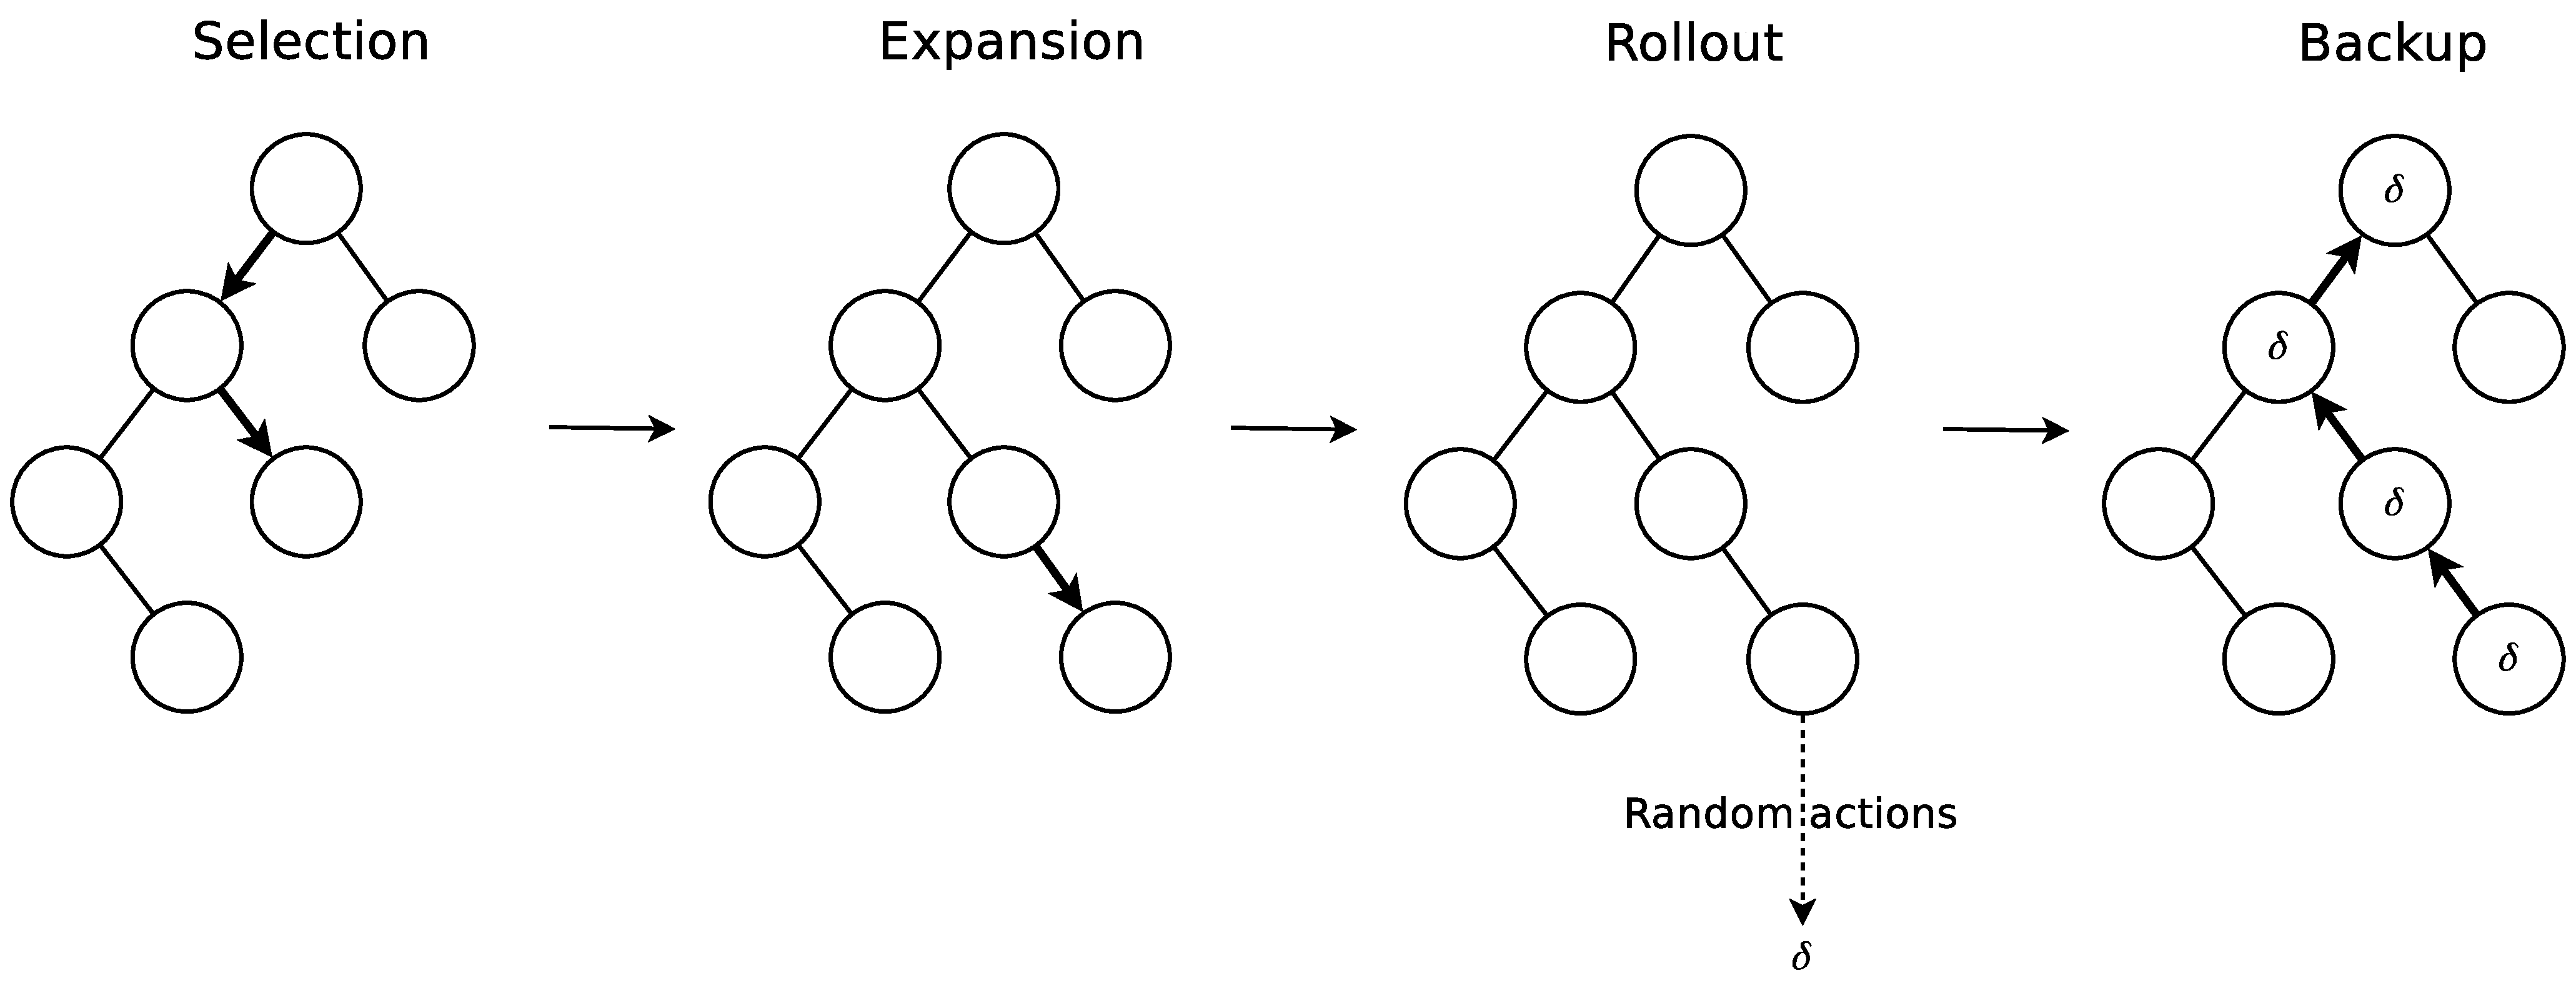
\epsfig{file=includes/mcts-wide.eps, width=\textwidth}
	\caption{One Monte Carlo tree search iteration}
	\label{fig:mcts}
\end{figure}

This section explains how MCTS approximates action values for states.  A tree is
built incrementally from the states and actions that are visited in a game. Each
node in the tree represents a state and each connection in the tree represents
an action taken in that state leading to a new state, which is represented by
the next tree node.  The process, as explained in Figure \ref{fig:mcts},
consists of four phases that are constantly repeated. It is started with the
current game state, which is represented by the root node of the tree. The first
action is chosen by an \emph{expansion strategy} and subsequently simulated,
resulting in a new game state, for which a new node is created. After expansion,
a \emph{rollout} is done from the new node, which means that a simulation is run
from the new node applying random actions until a predefined stop criterion is
met or the game ends. Finally, the score difference resulting from the rollout
is \emph{backed up} to the root node, which means that the reward is saved to the
visited nodes.  Then a new iteration starts. When all actions are expanded in a
node, that node is deemed \emph{fully expanded} and uses a \emph{selection
strategy} to select a next node. When a node is selected that is not fully
expanded, the expansion strategy is used to create a new node, after which a
rollout takes place and the results are backed up thereafter.

The selection strategy selects optimal actions in internal tree nodes, by
analyzing the values of their child nodes. An effective and very popular
selection strategy is the \emph{upper confidence tree (UCT)}
\cite{kocsis2006bandit}, which balances the choice between poorly explored
actions with a high uncertainty about their value and actions that have been
explored extensively, but have a higher value. A child node $j$ is selected to
maximize
\begin{equation}
	\label{eq:uct}
	UCT = v_{s'} C_p \sqrt{\frac{2 \ln n_s}{n_{s'}}}
\end{equation}
Where $v_{s'}$ is the value of child $s'$ as calculated by the backup function,
$n_s$ is the number of times the current node $s$ has been visited, $n_{s'}$ is
the number of times child $s'$ has been visited and $C_p > 0$ is a constant,
often set to $\sqrt{2}$, that shifts priority from exploration to exploitation.

The traditional expansion strategy is to explore each action at least once in
each node. After all actions have been expanded, the node applies the selection
strategy for further exploration. Some variants of MCTS reduce the branching
factor of the tree by only expanding the nodes selected by a special expansion
strategy. A specific example is the \emph{crazy stone} algorithm
\cite{coulom2007efficient}, which is an expansion strategy that was designed
specifically for Go. We will use an adaptation of this strategy in the algorithm
proposed in Chapter \ref{sec:learning}.  When using crazy stone, an action $i$
is selected with a probability proportional to $u_i$
\begin{equation}
	\label{eq:crazystone}
	u_i = \exp\left(K \frac{\mu_0 - \mu_i}{\sqrt{2\left(\sigma_0^2 +
\sigma_i^2\right)}}\right) + \epsilon_i
\end{equation}
Each action has an estimated value $\mu_i$ ordered in such a way that $\mu_0 >
\mu_1 > \ldots > \mu_N$, and a variance $\sigma_i^2$. $\epsilon_i$ prevents 
the probability of selecting a move to reach zero and its value is proportional to
the ordering of the expected values of the possible actions. K is a constant
that influences the exploration/exploitation trade off.
\begin{equation}
	\label{eq:epsilon}
	\epsilon_i = \frac{0.1 + 2^{-i} + a_i}{N}
\end{equation}
Where $a_i$ is 1 when an action is \emph{an atari move}, a go-specific
move that can otherwise easily be underestimated by MCTS, and otherwise 0.

After a rollout, the reward is backed up, which means that the estimated value
for every node that has been visited in this iteration is updated with the
reward of this simulation. Usually the estimated value of a node is the average
of all rewards backed up to that node.

\section{Q-learning}
\label{subsec:qlearning}
Q-learning is a relatively simple model free temporal difference learning method
that was proposed in 1992 \cite{watkins1992q}. The \emph{Q-value} of an action
for a state, $Q(s, a)$, is the discounted reward that can be achieved by
applying action $a$ to state $s$ and following the optimal policy afterwards. By
learning Q-values for every action in every state, it can estimate an optimal
policy. 

The general idea of Q-learning is to incrementally save the reward from the MDP,
in combination with the current Q-value of the state-action pair: the update
function uses the reward and the maximum of the Q-values of the next state. By
always using the maximum value of the next state as well, the Q-value function
will eventually converge to a depiction of the maximum future reward for a
state-action pair. More specifically, the update function for a state-action
pair is
\begin{equation}
	\label{eq:qlearning}
	Q(s, a) \gets Q(s, a) + \alpha \left(r + \gamma \max_{a \in A} Q(s', a) - Q(s, a)\right),
\end{equation}
where $r$ is the reward that is achieved by using action $a$ in state $s$,
leading to state $s'$. The algorithm has two parameters: $\gamma$ is the
discount factor, which indicates the importance of future states. $\alpha$ is the
learning rate, which determines how quickly the Q-values are updated.
Q-learning is shown to converge, even in problems with a stochastic transition
function, if $\alpha$, $\alpha$ decreases over time. In practice, however, it is
often set to $0.1$. The Q-table can be used to find the optimal policy by, for
each state $s$, selecting the action $a$ that maximizes $Q(s, a)$. Because after
each action only one state-action pair is being updated, Q-learning can take a
long time to converge, but it is guaranteed to converge to the optimal policy,
given that during exploration, each state-action pair is visited an infinite
number of times.

\section{Options}
\label{subsec:options}
In order to mimic human game playing strategies, defining subgoals and subtask,
we use options. Options have been proposed by Sutton et al.
\cite{sutton1999between} as a method to incorporate temporal abstraction in
field of reinforcement learning. A lot of progress has been made since, but a
lot of the research seems to focus on learning algorithms and little work is
done on combining options with tree search methods \cite{barto2003recent}, which
offer a model free planning framework.

An option is a predefined method of reaching a specific subgoal. Formally, it is
a triple $\langle I, \pi, \beta\rangle$ in which $I \subseteq S$ is an
initiation set, $\pi: S \times A \rightarrow [0, 1]$ is a policy and $\beta: S^+
\rightarrow[0,1]$ is a termination condition.  A policy $\pi$ defines the action
that should be taken in a state. The initiation set $I$ is a set of states in
which the option can be started. Typically, when the option starts, policy $\pi$
will be followed, until a state is reached that satisfies a termination
condition in $\beta$. After that, a new option is chosen and followed. 

Using options in an MDP removes the Markov property for that process: the state
information alone is no longer enough to predict an agent's actions, since the
actions are now not only state-dependant, but dependant on what option the agent
has chosen in the past as well. According to \cite{sutton1999between}, we can
now view the process as a \emph{semi-Markov decision process (SMDP)}
\cite{duff1995reinforcement}, where options are viewed as actions of variable
length. In this thesis, we will keep calling the original action set of the MDP
$A$, and the set of options $O$.  Normal actions can be treated as options as
well.  An option for action $a \in A$ has a initiation set $I = S$, the policy
$\pi$ is taking action $a$ in all the states.  The termination condition $\beta$
is that action $a$ should be performed once.


\section{Video Game Description Language}
\label{subsec:vgdl}
In order to test algorithms on several different games, a framework is used that
can access a large number of games in a similar manner. The GVGAI competition
uses the \emph{video game description language (VGDL)} \cite{schaul2013video},
in which games can be defined easily. VGDL aims to be a description language
for games that is clear, human readable and unambiguous. Games are easy to parse
and it is possible to automatically generate them. Using a VGDL framework,
algorithms can access all the games in a similar manner, resulting in a fair
method to compare their performances on several games.

To define a game in VGDL, two files are required. Firstly, the game description
should be made, which defines for each type of object what character in the
level description it corresponds to, what it looks like in a game visualization,
how it interacts with the rest of the game, and when it disappears from the
game. Secondly, a level description file is needed, in which each character maps
to an object in the game. The location in the file corresponds to its grid
location in the game. By defining these two files, a wide spectrum of games
can be created. A more extensive explanation of VGDL can be found in Chapter
\ref{subsec:games}.

In this thesis, we will use a Java implementation made for the GVGAI
competition, which comes with many games. In this version, algorithms only
observe the game information: score, game tick (timestep), the set of possible
actions and information about if the game is over and if the player won; Avatar
information: its position, orientation, speed and resources; and screen
information: Which sprites are on what location of the screen, and the size (in
pixels) of the game grid's blocks.

The algorithm proposed in this thesis will be
benchmarked on these games, using the rules of the GVGAI competition. 
This means that the algorithms do not have any access to the game and level
descriptions. When an algorithms starts playing a game, it typically knows
nothing of the game, except for the observation described above.
